% -*- TeX -*-
\documentclass[aspectratio=169,hyperref=colorlinks]{beamer}
%\documentclass[apectratio=34,hyperref=colorlinks]{beamer}

\usepackage{mathtools}
\usepackage{bm}
\usepackage{listings}

\usepackage{tikz}
\usetikzlibrary{shapes,arrows,calc}
\usetikzlibrary{decorations.pathreplacing}
\usetikzlibrary{fit,matrix}

\title{An overview of PyLith}
\subtitle{Plus a preview of multiphysics and other features coming in v3.0}
\author{Brad Aagaard}
\institute{
\includegraphics[scale=0.3]{../logos/USGSL}}
\date{April 13, 2017}

% ---------------------------------------------------- CUSTOMIZATION
%\renewcommand{\thispdfpagelabel}[1]{}
\usetheme{Logo}

\newcommand{\includefigure}[2][]{{\centering\includegraphics[#1]{#2}\par}}
\newcommand{\highlight}[1]{{\bf\usebeamercolor[fg]{structure}#1}}
\setbeamercolor{alerted text}{fg=ltgreen}

\usefonttheme[onlymath]{serif}
\newcommand{\lhs}[1]{{\color{blue}#1}}
\newcommand{\rhs}[1]{{\color{red}#1}}
\newcommand{\annotateL}[2]{%
  {\color{blue}\underbrace{\color{blue}#1}_{\color{blue}\mathclap{#2}}}}
\newcommand{\annotateR}[2]{%
  {\color{red}\underbrace{\color{red}#1}_{\color{red}\mathclap{#2}}}}
\newcommand{\trialvec}[1][]{{\vec{\psi}_\mathit{trial}^{#1}}}
\newcommand{\trialscalar}[1][]{{\psi_\mathit{trial}^{#1}}}
\newcommand{\basisvec}[1][]{{\vec{\psi}_\mathit{basis}^{#1}}}
\newcommand{\basisscalar}[1][]{{\psi_\mathit{basis}^{#1}}}

\newcommand{\tensor}[1]{\bm{#1}}

% Colors
\definecolor{ltorange}{rgb}{1.0, 0.74, 0.41} % 255/188/105
\definecolor{orange}{rgb}{0.96, 0.50, 0.0} % 246/127/0

\definecolor{ltred}{rgb}{1.0, 0.25, 0.25} % 255/64/64
\definecolor{red}{rgb}{0.79, 0.00, 0.01} % 201/0/3

\definecolor{ltpurple}{rgb}{0.81, 0.57, 1.00} % 206/145/255
\definecolor{purple}{rgb}{0.38, 0.00, 0.68} % 97/1/175

\definecolor{ltblue}{rgb}{0.2, 0.73, 1.0} % 51/187/255
\definecolor{mdblue}{rgb}{0.28, 0.50, 0.80} % 72/128/205
\definecolor{blue}{rgb}{0.12, 0.43, 0.59} % 30/110/150

\definecolor{ltltgreen}{rgb}{0.7, 1.00, 0.7} % 96/204/14
\definecolor{ltgreen}{rgb}{0.37, 0.80, 0.05} % 96/204/14
\definecolor{green}{rgb}{0.23, 0.49, 0.03} % 59/125/8
  
\definecolor{dkslate}{rgb}{0.18, 0.21, 0.28} % 47/53/72
\definecolor{mdslate}{rgb}{0.45, 0.50, 0.68} % 114/127/173
\definecolor{ltslate}{rgb}{0.85, 0.88, 0.95} % 216/225/229


% .cfg
\lstdefinelanguage{cfg}{%
  basicstyle=\tiny\ttfamily,
  frame=tb,%
  morecomment=[l][\color{orange}\itshape]{\#},
  morecomment=[l][\color{orange}\itshape]{;},
  moredelim=[is][\color{red}\bfseries]{<h>}{</h>},
  moredelim=[is][\color{purple}\bfseries]{<p>}{</p>},
  moredelim=[is][\color{blue}\bfseries]{<f>}{</f>},
}
\lstnewenvironment{cfg}{\lstset{language=cfg}}{}


% --------------------------------------------------------- DOCUMENT
\begin{document}

% ------------------------------------------------------------ SLIDE
\maketitle

\logo{
\includegraphics[height=4.5ex]{../logos/cig_blackfg}}

% ========================================================== SECTION
\section{Introduction}

% ------------------------------------------------------------ SLIDE
\begin{frame}
  \frametitle{PyLith}
  \summary{A modern, community-driven code for crustal deformation modeling}
  
  \begin{itemize}
  \item Developers
    \begin{itemize}
    \item Brad Aagaard (USGS)
    \item Matthew Knepley (Rice University)
    \item Charles Williams (GNS Science)
    \end{itemize}
  \item Combined dynamic modeling capabilities of EqSim (Aagaard) with
    the quasi-static modeling capabilities of Tecton (Williams)
  \item Use modern software engineering  to develop an open-source,
    community code 
    \begin{itemize}
    \item Modular design
    \item Testing
    \item Documentation
    \item Distribution
    \end{itemize}
  \item PyLith v1.0 was released in 2007
  \end{itemize}

  \vspace*{-2.5cm}\hspace{0.5\textwidth}\includefigure[height=3.0cm]{figs/downloads}

\end{frame}


% ------------------------------------------------------------ SLIDE
\begin{frame}
  \frametitle{Crustal Deformation Modeling}
  \summary{Elasticity problems where geometry does not change significantly}

  \vfill
  Quasi-static modeling associated with earthquakes
  \vfill

  \begin{itemize}
  \item Strain accumulation associated with interseismic deformation
    \begin{itemize}
    \item What is the stressing rate on faults X and Y?
    \item Where is strain accumulating in the crust?
    \end{itemize}
  \item Coseismic stress changes and fault slip
    \begin{itemize}
    \item What was the slip distribution in earthquake A?
    \item How did earthquake A change the stresses on faults X and Y?
    \end{itemize}
  \item Postseismic relaxation of the crust
    \begin{itemize}
    \item What rheology is consistent with observed postseismic deformation?
    \item Can aseismic creep or afterslip explain the deformation?
    \end{itemize}
  \end{itemize}
  \vfill

\end{frame}


% ------------------------------------------------------------ SLIDE
\begin{frame}
  \frametitle{Crustal Deformation Modeling}
  \summary{Elasticity problems where geometry does not change significantly}

  \vfill
  Dynamic modeling associated with earthquakes
  \vfill

  \begin{itemize}
  \item Modeling of strong ground motions
    \begin{itemize}
    \item Forecasting the amplitude and spatial variation in ground
      motion for scenario earthquakes
    \end{itemize}
  \item Coseismic stress changes and fault slip
    \begin{itemize}
    \item How did earthquake A change the stresses on faults X and Y?
    \end{itemize}
  \item Earthquake rupture behavior
    \begin{itemize}
    \item What fault constitutive models/parameters are consistent
      with the observed rupture propagation in earthquake A?
    \end{itemize}
  \end{itemize}
  \vfill

\end{frame}


% ------------------------------------------------------------ SLIDE
\begin{frame}
  \frametitle{Crustal Deformation Modeling}
  \summary{Elasticity problems where geometry does not change significantly}

  \vfill
  Volcanic deformation associated with magma chambers and/or dikes
  \begin{itemize}
  \item Inflation
    \begin{itemize}
    \item What is the geometry of the magma chamber?
    \item What is the potential for an eruption?
    \end{itemize}
  \item Eruption
    \begin{itemize}
    \item Where is the deformation occurring?
    \item What is the ongoing potential for an eruption?
    \end{itemize}
  \item Dike intrusions
    \begin{itemize}
    \item What is the geometry of the intrusion?
    \item What is the pressure change and/or amount of opening/dilatation?
    \end{itemize}
  \end{itemize}
  \vfill

\end{frame}


% ------------------------------------------------------------ SLIDE
\begin{frame}
  \frametitle{Crustal Deformation Modeling}
  \summary{Overview of workflow for typical research problem}

  \includefigure[height=7.2cm]{figs/workflow}
  
\end{frame}


% ========================================================== SECTION
\subsection{Governing Equations}

% ------------------------------------------------------------ SLIDE
\begin{frame}
  \frametitle{Governing Equations}
  \summary{}

  \vfill
  Elasticity equation
  \begin{gather}
    \sigma_{ij,j} + f_i = \rho \ddot{u} \text{ in } V, \\
    \sigma_{ij} n_j = T_i \text{ on } S_T, \\
    u_i = u_i^0 \text{ on } S_u, \text{ and } \\
    R_{ki}(u^{+}_i - u^{-}_i) = d_k \text{ on } S_f.
  \end{gather}
  Multiply by weighting function and integrate over the volume,
  \begin{equation}
    -\int_V (\sigma_{ij,j} + f_i - \rho \ddot{u}_i) \phi_i \, dV = 0
  \end{equation}
  After some algebra,
  \begin{equation}
    -\int_V \sigma_{ij} \phi_{i,j} \, dV 
    + \int_{S_T} T_i \phi_i\, dS
    + \int_V f_i \phi_i \, dV 
    - \int_V \rho \ddot{u}_i \phi_i \, dV = 0
  \end{equation}
  \vfill
  
\end{frame}


% ------------------------------------------------------------ SLIDE
\begin{frame}
  \frametitle{Discretize Domain Using Finite Elements}
   \summary{PyLith v2.0.0 and later use interpolated meshes}
 
   \begin{center}
     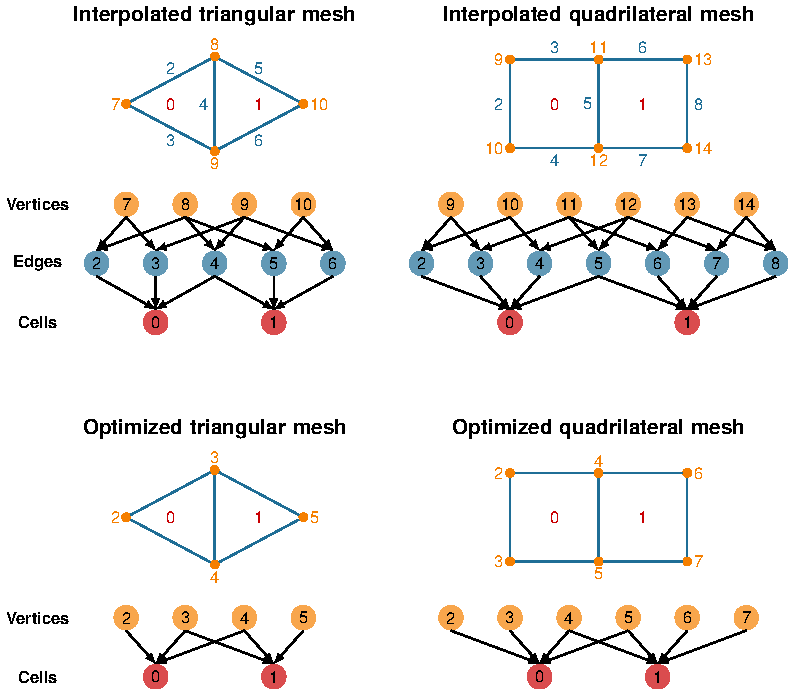
\includegraphics[height=7.0cm]{figs/meshtopology}
   \end{center}
   
 \end{frame}
 

% ========================================================== SECTION
\section{Using PyLith}

% ------------------------------------------------------------ SLIDE
\begin{frame}
  \frametitle{Overview of PyLith Workflow}
  \summary{}

  \includefigure[height=7.2cm]{figs/runpylith}
\end{frame}

% ------------------------------------------------------------ SLIDE
\begin{frame}
  \frametitle{PyLith as a Hierarchy of Components}
  \summary{Components are the basic building blocks}

  \begin{minipage}{0.53\textwidth}
    \begin{itemize}
    \item Separate functionality into discrete modules (components)
    \item Alternative implementations use the same interfaces to allow plug-n-play
    \item Top-level interfaces in Python with computational code in C++
      \begin{itemize}
      \item Python dynamic typing permits adding new modules at runtime.
      \item Users can add functionality without modifying the PyLith code.
      \end{itemize}
    \end{itemize}
  \end{minipage}\hfill
  \begin{minipage}{0.43\textwidth}
    \includefigure[height=5cm]{figs/component}
  \end{minipage}

\end{frame}

% ------------------------------------------------------------ SLIDE
\begin{frame}[fragile]
  \frametitle{Parameter Files}
  \summary{Simple syntax for specifying parameters for properties and components}

\begin{cfg}
# Syntax
<h>[pylithapp.COMPONENT.SUBCOMPONENT]</h> ; Inline comment
<f>COMPONENT</f> = OBJECT
<p>PARAMETER</p> = VALUE

# Example
<h>[pylithapp.mesh_generator]</h> ; Header indicates path of mesh_generator in hierarchy
<f>reader</f> = pylith.meshio.MeshIOCubit ; Use mesh from CUBIT/Trelis
<p>reader.filename</p> = mesh_quad4.exo ; Set filename of mesh.
<p>reader.coordsys.space_dim</p> = 2 ; Set coordinate system of mesh.

<h>[pylithapp.problem.solution_outputs.output]</h> ; Set output format
<f>writer</f> = pylith.meshio.DataWriterHDF5
<p>writer.filename</p> = axialdisp.h5

<h>[pylithapp.problem]</h>
<f>bc</f> = [x_neg, x_pos, y_neg] ; Create array of boundary conditions
<f>bc.x_neg</f> = pylith.bc.DirichletTimeDependent ; Set type of boundary condition
<f>bc.x_pos</f> = pylith.bc.DirichletTimeDependent
<f>bc.y_neg</f> = pylith.bc.DirichletTimeDependent

<h>[pylithapp.problem.bc.x_pos]</h> ; Boundary condition for +x
<p>constrained_dof</p> = [0] ; Constrain x DOF
<p>label</p> = edge_xpos ; Name of nodeset from CUBIT/Trelis
<f>db_auxiliary_fields</f> = spatialdata.spatialdb.SimpleDB ; Set type of spatial database
<p>db_auxiliary_fields.label</p> = Dirichlet BC +x edge
<p>db_auxiliary_fields.iohandler.filename</p> = axial_disp.spatialdb ; Filename for database
\end{cfg}

\end{frame}

% ------------------------------------------------------------ SLIDE
\begin{frame}
  \frametitle{Parameters Graphical User-Interface}
  \summary{{\tt cd parametersgui; ./pylith\_paramviewer}}

  \includefigure[height=8.5cm]{figs/paramgui_snapshot}

\end{frame}

% ------------------------------------------------------------ SLIDE
\begin{frame}
  \frametitle{Spatial Databases}
  \summary{User-specified field/value in space for properties and BC values.}

  \begin{itemize}
 \item Examples
    \begin{itemize}
    \item Uniform value for Dirichlet BC (0-D)
    \item Piecewise linear variation in tractions for Neumann BC (1-D)
    \item SCEC CVM-H seismic velocity model (3-D)
    \end{itemize}
  \item Generally independent of discretization for problem
  \item Available spatial databases
    \begin{description}
    \item[UniformDB] Optimized for uniform value
    \item[SimpleDB] Arbitrarily distributed points for variations in 0-D, 1-D, 2-D, or 3-D
    \item[SimpleGridDB] Logically gridded points for variations in 0-D, 1-D, 2-D, or 3-D
    \item[SCECCVMH] SCEC CVM-H seismic velocity model v5.3
    \item[ZeroDispDB] Special case of UniformDB
    \end{description}
 \end{itemize}

\end{frame}

% ------------------------------------------------------------ SLIDE
\begin{frame}
  \frametitle{PyLith Design: Focus on Geodynamics}
  \summary{Leverage packages developed by computational scientists}

  \includefigure[height=7.0cm]{figs/packages}

\end{frame}

% ------------------------------------------------------------ SLIDE
\begin{frame}
  \frametitle{PyLith Development Follows CIG Best Practices}
  \summary{\href{https://github.com/geodynamics/best\_practices}{github.com/geodynamics/best\_practices}}

  \begin{itemize}
  \item Version Control
    \begin{itemize}
    \item New features are added in separate branches.
    \item Use 'master' branch as stable development branch.
    \end{itemize}
  \item Coding
    \begin{itemize}
    \item User-friendly specification of parameters at runtime.
    \item Development plan, updated annually.
    \item Users can add features or alternative implementations without modifying code.
    \end{itemize}
  \item Portability
    \begin{itemize}
    \item Build procedure is independent of compilers and optimization flags.
    \item Multiple builds (debug/optimized) from same source.
    \end{itemize}
  \item Documentation and User Workflow
    \begin{itemize}
    \item Extensive example suite with varying levels of complexity.
    \item Changing simulation parameters does not require rebuilding.
    \item Displays version information via {\tt --version} command line argument.
    \end{itemize}
  \end{itemize}

\end{frame}

% ------------------------------------------------------------ SLIDE
\begin{frame}
  \frametitle{Development Tools}
  \summary{Leverage open-source tools for efficient code development.}

  \begin{description}
  \item[GitHub] Code repository supporting simultaneous, independent implementation of new features.
  \item[Doxygen] Document parameters and purpose of every object and its functions.
  \item[CppUnit] Test nearly every function in code during development.
  \item[Travis CI \& Jenkins] Run tests when code is committed to repository.
  \item[gcov] Records which lines of code tests cover.
  \end{description}

\end{frame}

% ------------------------------------------------------------ SLIDE
\begin{frame}
  \frametitle{Testing}
  \summary{Multiple levels of testing facilitates identifying bugs at origin.}

  \begin{description}
  \item[unit tests] Serial testing at level of single and multiple functions.
  \item[full-scale tests] Serial and parallel pass/fail tests of full problems using Method of Manufactured Solutions.
  \item[benchmarks] Serial and parallel tests for code comparisons, etc.
  \end{description}

\end{frame}

% ------------------------------------------------------------ SLIDE
\begin{frame}
  \frametitle{PyLith Current Release: v2.2.0 (Mar 31, 2017)}
  \summary{}

  \begin{itemize}
  \item Time integration schemes and elasticity formulations
    \begin{itemize}
    \item Implicit for quasistatic problems (neglect inertial terms)
      \begin{itemize}
      \item Infinitesimal strains
      \item Small strains
      \end{itemize}
    \item Explicit for dynamic problems
      \begin{itemize}
      \item Infinitesimal strains
      \item Small strains
      \item Numerical damping via viscosity
     \end{itemize}
    \end{itemize}
  \item Bulk constitutive models (2-D and 3-D)
    \begin{itemize}
    \item Elastic model 
    \item Linear Maxwell viscoelastic models
    \item Generalized Maxwell viscoelastic models
    \item Power-law viscoelastic model
    \item Drucker-Prager elastoplastic model
    \end{itemize}
 \end{itemize}

\end{frame}


% ------------------------------------------------------------ SLIDE
\begin{frame}
  \frametitle{Features in PyLith v2.2 (cont.)}
  \summary{}

  \begin{itemize}
  \item Boundary and interface conditions
    \begin{itemize}
    \item Time-dependent Dirichlet boundary conditions
    \item Time-dependent Neumann (traction) boundary conditions
    \item Absorbing boundary conditions
    \item Kinematic (prescribed slip) fault interfaces w/multiple ruptures
    \item Dynamic (friction) fault interfaces
    \item Fault interfaces with T intersections
    \item Time-dependent point forces
    \item Gravitational body forces
    \end{itemize}
  \item Fault constitutive models
    \begin{itemize}
    \item Static friction
    \item Linear slip-weakening
    \item Linear time-weakening
    \item Dieterich-Ruina rate and state friction w/ageing law
   \end{itemize}
 \end{itemize}

\end{frame}


% ------------------------------------------------------------ SLIDE
\begin{frame}
  \frametitle{Features in PyLith v2.2 (cont.)}
  \summary{}

  \begin{itemize}
  \item Automatic and user-controlled time stepping
  \item Ability to specify initial stress/strain state
  \item Importing meshes
    \begin{itemize}
    \item LaGriT: GMV/Pset
    \item CUBIT/Trelis: Exodus II
    \item ASCII: PyLith mesh ASCII format (intended for toy problems only)
    \end{itemize}
  \item Output: VTK and HDF5 files
    \begin{itemize}
    \item Solution over volume
    \item Solution over surface boundary
    \item Solution interpolated to user-specified points w/station names
    \item State variables (e.g., stress and strain) for each material
    \item Fault information (e.g., slip and tractions)
    \end{itemize}
 \end{itemize}
  
\end{frame}


% ------------------------------------------------------------ SLIDE
\begin{frame}
  \frametitle{Features in PyLith v2.2 (cont.)}
  \summary{}

  \begin{itemize}
  \item Automatic conversion of units for all parameters
  \item Parallel uniform global refinement
  \item PETSc linear and nonlinear solvers
    \begin{itemize}
    \item Custom preconditioner with algebraic multigrid solver
    \end{itemize}
  \item Output of simulation progress estimates runtime
 \end{itemize}
  
\end{frame}


% ========================================================== SECTION
\subsection{Fault Implementation}

% ------------------------------------------------------------ SLIDE
\begin{frame}[fragile]
  \frametitle{Fault Interface}
  \summary{Fault tractions couple deformation across interface}

  \includefigure[height=7.0cm]{figs/domaindecomp}

\end{frame}


% ------------------------------------------------------------ SLIDE
\begin{frame}
  \frametitle{Implementation: Fault Interfaces}
   \summary{Use zero volume/area cohesive cells to control fault behavior}
 
   \includefigure[height=6.2cm]{figs/cohesivecells}
   \vfill
   See Aagaard, Knepley, and Williams, JGR, 2013
   \href{http://dx.doi.org/10.1002/jgrb.50217}{doi:
     10.1002/jgrb.50217} for more information.
 \end{frame}
 

% ------------------------------------------------------------ SLIDE
\begin{frame}[fragile]
  \frametitle{Fault Implementation: Governing Equations}
  \summary{Terms in governing equation associated with fault}

  \begin{itemize}
  \item Tractions on fault surface are analogous to boundary tractions
    \tikz{
      \matrix [matrix of nodes, ampersand replacement=\&] {
      \node {$ \displaystyle \ldots $}; \&
      \node [below delimiter=\}] {$ \displaystyle + \int_{S_T} \vec{\phi} \cdot \vec{T} \, dS$}; \&
      \node [below delimiter=\}] {$ \displaystyle - \int_{S_{f^+}} \vec{\phi} \cdot \vec{l} \, dS$}; \&
      \node [below delimiter=\}] {$ \displaystyle + \int_{S_{f^-}} \vec{\phi} \cdot \vec{l} \, dS$}; \&
      \ldots = 0 \\
      \& \node {Neumann BC}; \& 
      \node {Fault +}; \&
      \node {Fault -}; \& \\
    };
}
  \item Constraint equation relates slip to relative displacement
    \tikz{
      \matrix [matrix of nodes, ampersand replacement=\&] {
        \node {$ \displaystyle \int_{S_f} \vec{\phi} \cdot ($}; \&
        \node [below delimiter=\}] {$\displaystyle\vec{d}$}; \&
        \node {$ \displaystyle - $}; \&
        \node [below delimiter=\}] {$ \displaystyle (\vec{u}_{+} - \vec{u}_{-}) $}; \&
        \node {$ \displaystyle ) dS = 0 $}; \\
        \& Slip \& \& Relative Disp. \& \\
    };
}
  \end{itemize}

\end{frame}


% ------------------------------------------------------------ SLIDE
\begin{frame}
  \frametitle{Fault Slip Implementation}
  \summary{Use Lagrange multipliers to specify slip}

  \begin{itemize}
  \item System without cohesive cells
    \begin{itemize}
    \item Conventional finite-element elasticity formulation
      \begin{equation}
        \underbar{A} \vec{u} = \vec{b} \nonumber
      \end{equation}
    \item Fault slip associated with relative displacements across fault
      \begin{equation}
        \underbar{C} \vec{u} = \vec{d} \nonumber
      \end{equation}
    \end{itemize}
  \item System with Lagrange multiplier constraints for fault slip
    \begin{equation}
      \left( \begin{array}{cc}
          \underbar{A} & \underbar{C}^T\\
          \underbar{C} & 0
        \end{array} \right)
      \left( \begin{array}{c}
          \vec{u}\\
          \vec{l}
        \end{array}\right)
      =
      \left( \begin{array}{c}
          \vec{b}\\
          \vec{d}
        \end{array} \right)
      \nonumber
    \end{equation}
  \item Prescribed (kinematic) slip\\
    Specify fault slip ($\vec{d}$) and solve for Lagrange multipliers ($\vec{l}$)
  \item Spontaneous (dynamic) slip\\
    Adjust fault slip to be compatible with fault constitutive model
\end{itemize}
  
\end{frame}


% ------------------------------------------------------------ SLIDE
\begin{frame}
  \frametitle{Implementing Fault Slip with Lagrange multipliers}
 
 \begin{itemize}
 \item Advantages
   \begin{itemize}
   \item Fault implementation is local to cohesive cell
   \item Solution includes tractions generating slip (Lagrange multipliers)
   \item Retains block structure of matrix, including symmetry
   \item Offsets in mesh mimic slip on natural faults
   \end{itemize}
 \item Disadvantages 
   \begin{itemize}
   \item Cohesive cells require adjusting topology of finite-element
     mesh
   \item Scalable preconditioner/solver is more complex
  \end{itemize}
 \end{itemize}
  
\end{frame}


% ========================================================== SECTION
\section{PyLith v3.0}

% ------------------------------------------------------------ SLIDE
\begin{frame}
  \frametitle{PyLith v3.0}
  \summary{}

  \begin{itemize}
  \item Multiphysics through pointwise integration kernels
  \item Higher order spatial and temporal discretizations
  \item Adaptive time stepping via PETSc TS
  \item Improved fault formulation for spontaneous rupture (v3.1)
  \end{itemize}

\end{frame}

\abovedisplayskip=2pt
\abovedisplayshortskip=2pt
\belowdisplayskip=2pt
\belowdisplayshortskip=2pt

% ------------------------------------------------------------ SLIDE
\begin{frame}
  \frametitle{Aside: Finite-Element Method}
  \summary{Strong form to weak form}

  Solve governing equation in integrated sense:
  \begin{equation}
    \int_\Omega \trialscalar \cdot \mathit{PDE} \, d\Omega = 0,
  \end{equation}
  by minimizing the error with respect to the unknown coefficients.
  \vfill
  This leads to equations of the form:
  \begin{equation}
    \int_\Omega \trialscalar \cdot f_0(x,t) + \nabla \trialscalar \cdot f_1(x,t) \, d\Omega = 0.
  \end{equation}

\end{frame}

% ------------------------------------------------------------ SLIDE
\begin{frame}
  \frametitle{Governing Equations}
  \summary{}

  We want to solve equations in which the weak form can be expressed
  as
  \begin{gather}
    \lhs{F(t,s,\dot{s})} = \rhs{G(t,s)} \\
    s(t_0) = s_0
  \end{gather}
  where $\lhs{F}$ and $\rhs{G}$ are vector functions, $t$ is time, and $s$ is the solution vector.
  \vfill
  Using the finite-element method and divergence theorem, we cast the weak form into
  \begin{multline}
    \int_\Omega \trialvec \cdot \lhs{\vec{f}_0(t,s,\dot{s})} + \nabla \trialvec : \lhs{\tensor{f}
    _1(t,s,\dot{s})} \, 
    d\Omega = \\
    \int_\Omega \trialvec \cdot \rhs{\vec{g}_0(t,s)} + \nabla \trialvec : \rhs{\tensor{g}_1(t,s)} \, 
    d\Omega,
  \end{multline}
  where $\vec{f}_0$ and $\vec{g}_0$ are vectors, and $\tensor{f}_1$ and
  $\tensor{g}_1$ are tensors.

\end{frame}

% ------------------------------------------------------------ SLIDE
\begin{frame}
  \frametitle{Explicit Time Stepping}
  \summary{}

  Explicit time stepping with the PETSc TS requires $\lhs{F(t,s,\dot{s})} = \dot{s}$.
  \vfill
  Normally $\lhs{F(t,s,\dot{s})}$ contains the inertial term ($\rho \ddot{u}$).
  \vfill
  Therefore, when using explicit time stepping we transform our equation into the form:
  \begin{align}
    \lhs{F^*(t,s,\dot{s})} = \lhs{\dot{s}} &= \rhs{G^*(t,s)} \\
    \lhs{\dot{s}} &= \lhs{M^{-1}}\rhs{G(t,s)}.
  \end{align}  

\end{frame}

% ------------------------------------------------------------ SLIDE
\begin{frame}
  \frametitle{Solving the Equations}
  \summary{Explicit time stepping requires a subset of the terms used in implicit time stepping.}

  \begin{itemize}
  \item PETSc TS object provides time-stepping and solver implementations
    \begin{itemize}
    \item Application code provides functions for computing RHS and LHS residuals and Jacobians
    \end{itemize}
  \item Explicit time stepping
    \begin{itemize}
    \item Compute RHS residual, $\rhs{G(t,s)}$
    \item Compute lumped inverse of LHS, $\lhs{M^{-1}}$
    \item No need to compute LHS residual, because $\lhs{F(t,s,\dot{s})} = \dot{s}$
    \end{itemize}
  \item Implicit time stepping (Krylov solvers)
    \begin{itemize}
    \item Compute RHS residual, $\rhs{G(t,s)}$
    \item Compute LHS residual, $\lhs{F(t,s,\dot{s})}$
    \item Compute RHS Jacobian, $\rhs{J_G}$ = $\rhs{\frac{\partial G}{\partial s}}$
    \item Compute LHS Jacobian, $\lhs{J_F}$ = $\lhs{\frac{\partial F}{\partial s}} + t_\mathit{shift}\lhs{\frac{\partial F}{\partial \dot{s}}}$
    \end{itemize}
  \end{itemize}

\end{frame}

% ------------------------------------------------------------ SLIDE
\begin{frame}
  \frametitle{Example: Elasticity}
  \summary{}

      \begin{align}
        \lhs{\rho \frac{\partial^2\vec{u}}{\partial t^2}} &= \rhs{\vec{f}(\vec{x},t) + \tensor{\nabla} \cdot \tensor{\sigma}(\vec{u})} \text{ in } \Omega, \\
        %
        \tensor{\sigma} \cdot \vec{n} &= \vec{\tau}(\vec{x},t) \text{ on } \Omega_\tau, \\
        %
        \vec{u} &= \vec{u}_0(\vec{x},t) \text{ on } \Omega_u,
      \end{align}

      \vfill

      {\bf Implicit Time Stepping without Inertia}

      Displacement $\vec{u}$ is the unknown, $\vec{s}= \vec{u}$.
      \begin{align}
        \annotateL{0}{\vec{f}_0^u} &=
  \int_\Omega \trialvec[u] \cdot \annotateR{\vec{f}(\vec{x},t)}{\vec{g}_0^u} + \nabla \trialvec[u] : \annotateR{-\tensor{\sigma}(\vec{u})}{\tensor{g}_1^u} \, d\Omega + \int_{\Omega_\tau} \trialvec[u] \cdot \annotateR{\vec{\tau}(\vec{x},t)}{\vec{g}_0^u} \, d\Omega_\tau
      \end{align}

      \vfill
      Different constitutive models are encapsulated in alternative
      kernels for $\tensor{\sigma}(\vec{u})$.

\end{frame}

% ------------------------------------------------------------ SLIDE
\begin{frame}
  \frametitle{Example: Elasticity (continued)}
  \summary{}

      {\bf Explicit Time Stepping with Inertia}

      Form a first order equation using displacement $\vec{u}$ and velocity $\vec{v}$ as
      unknowns, $\vec{s}^T = \left( \begin{array}{cc} \vec{u} & \vec{v} \end{array} \right)^T$
      \begin{align}
        \int_\Omega \trialvec[u] \cdot \annotateL{\frac{\partial \vec{u}}{\partial t}}{\dot{u}} \, d\Omega &= 
        \int_\Omega \trialvec[u] \cdot \annotateR{\vec{v}}{\vec{g}_0^u} \, d\Omega, \\
        %
        \int_\Omega \trialvec[v] \cdot \annotateL{\frac{\partial \vec{v}}{\partial t}}{\dot{v}} \, d\Omega &=
\frac{1}{\vec{m}} \left(
  \int_\Omega \trialvec[v] \cdot \annotateR{\vec{f}(\vec{x},t)}{\vec{g}_0^v} + \nabla \trialvec[v] : \annotateR{-\tensor{\sigma}(\vec{u})}{\tensor{g}_1^v} \, d\Omega + \int_{\Omega_\tau} \trialvec[v] \cdot \annotateR{\vec{\tau}(\vec{x},t)}{\vec{g}_0^v} \, d\Omega_\tau \right), \\
\vec{m} &= \int_\Omega \trialvec[v] \cdot {\annotateL{\rho}{J_{f0}^{vv}}} \basisvec[v] \, d\Omega
      \end{align}


\end{frame}

% ------------------------------------------------------------ SLIDE
\begin{frame}
  \frametitle{Example: Elasticity (continued)}
  \summary{Implementing the governing equations involves a small set of simple kernels.}

  {\centering
  \begin{tabular}{ccc}
    & {\bf Implicit} & {\bf Explicit} \\ \hline
    $\rhs{\vec{v}}$   &   --   &   $\rhs{\vec{g}_0^v}$ \\
    $\rhs{\vec{f}(\vec{x},t)}$   &   $\rhs{\vec{g}_0^u}$   &   $\rhs{\vec{g}_0^v}$ \\
    $\rhs{-\tensor{\sigma}(\vec{u})}$   & $\rhs{\tensor{g}_1^u}$   &   $\rhs{\tensor{g}_1^v}$ \\
    $\rhs{\vec{\tau}(\vec{x},t)}$   &   $\rhs{\vec{g}_0^u}$   &   $\rhs{\vec{g}_0^v}$ \\
    $\lhs{\vec{0}}$   &   $\lhs{\vec{f}_0^u}$ & -- \\
    $\lhs{\rho}$ & -- & $\lhs{J_{f_0}^{uv}}$ \\
    \hline
  \end{tabular}\par}
  \vfill
  We also have simple kernels for the Jacobians needed in implicit time stepping.

\end{frame}

% ------------------------------------------------------------ SLIDE
\begin{frame}
  \frametitle{Example: Poroelasticity Neglecting Inertia}
  \summary{}

        We assume a compressible fluid completely saturates a porous
        solid undergoing infinitesimal strain.

        Elasticity equilibrium equation neglecting inertia:
        \begin{alignat}{2}
          0 &= \rhs{\vec{f}(\vec{x},t) + \tensor{\nabla} \cdot \tensor{\sigma}(\vec{u},p_f)} \text{ in } \Omega, 
          & \quad
          \tensor{\sigma} \cdot \vec{n} = \vec{\tau}(\vec{x},t) \text{ on } \Omega_\tau, 
          %
          \vec{u} = \vec{u}_0(\vec{x},t) \text{ on } \Omega_u,
        \end{alignat}
        Mass balance of the fluid:
        \begin{alignat}{2}
          \lhs{\frac{\partial \zeta(\vec{u},p_f)}{\partial t}} = \rhs{\gamma(\vec{x},t) - \nabla \cdot \vec{q}(p_f)} \text{ in }\Omega,
          & \quad
          \vec{q} \cdot \vec{n} = q_0(\vec{x},t) \text{ on }\Omega_q,
          %
          p_f = p_0(\vec{x},t) \text{ on }\Omega_p,
        \end{alignat}
        Darcy's law:
        \begin{alignat}{2}
          \vec{q}(p_f) = -\kappa (\nabla p_f - \vec{f}_f), 
          & \quad
          \kappa = \frac{k}{\eta_f}
        \end{alignat}
        Constitutive behavior of the fluid:
        \begin{alignat}{2}
          \zeta(\vec{u},p_f) = \alpha (\nabla \cdot \vec{u}) + \frac{p_f}{M}, 
          & \quad
          \frac{1}{M} = \frac{\alpha-\phi}{K_s} + \frac{\phi}{K_f},
        \end{alignat}
        Constitutive behavior of the solid (linear elasticity):
        \begin{equation}
          \tensor{\sigma}(\vec{u},p_f) = \tensor{C} : \tensor{\epsilon} - \alpha p_f \tensor{I}
        \end{equation}


\end{frame}

% ------------------------------------------------------------ SLIDE
\begin{frame}
  \frametitle{Example: Poroelasticity Neglecting Inertia}
  \summary{}

      Consider displacement $\vec{u}$ and fluid pressure $p_f$ as
      unknowns, $\vec{s}^T = \left( \begin{array}{cc} \vec{u} & p_f \end{array} \right)^T$
      \begin{align}
        \annotateL{0}{\vec{f}_0^u} &= \int_\Omega \trialvec[u] \cdot \annotateR{\vec{f}(\vec{x},t)}{\vec{g}^u_0} + \nabla \trialvec[u] : \annotateR{-\tensor{\sigma}(\vec{u},p_f)}{\tensor{g}^u_1} \, d\Omega + \int_{\Omega_\tau} \trialvec[u] \cdot \annotateR{\vec{\tau}(\vec{x},t)}{\vec{g}^u_0} \, d\Omega_\tau, \\
%
 \int_\Omega  \trialscalar[p] \annotateL{\frac{\partial \zeta(\vec{u},p_f)}{\partial t}}{f^p_0} \, d\Omega &= 
 \int_\Omega \trialscalar[p] \annotateR{\gamma(\vec{x},t)}{g^p_0} + \nabla \trialscalar[p] \cdot \annotateR{\vec{q}(p_f)}{\vec{f}^p_1} \, d\Omega
 + \int_{\Omega_q} \trialscalar[p] \annotateR{(-q_0(\vec{x},t))}{g^p_0} \, d\Omega_q.
      \end{align}

      Poroelasticity involves many of the same kernels as elasticity plus a few additional ones.

\end{frame}

% ------------------------------------------------------------ SLIDE
\begin{frame}
  \frametitle{Finite-Element Discretization}
  \summary{Specify discretizations for solution fields and auxiliary fields}

  \begin{itemize}
  \item Solution Fields \\
    Specify basis functions and quadrature for each field in solution.
  \item Auxiliary Fields 
    \begin{itemize}
    \item Fields associated with parameters and state variables for constitutive models \& boundary conditions.
    \item Populated from spatial databases.
    \item Specify basis functions for each subfield in the auxiliary fields.
    \end{itemize}
  \item PETSc DMPlex infrastructure unpacks/packs
    information to/from solution and auxiliary fields and calling
    finite-element kernels.
  \end{itemize}


\end{frame}

% ------------------------------------------------------------ SLIDE
\begin{frame}
  \frametitle{Summary of Multiphysics Implementation}
  \summary{}

  We decouple the element definition from the fully-coupled equation,
  using pointwise kernels that look like the PDE.

  \vfill    
  \begin{description}
  \item[Flexibility] The cell traversal, handled by the library,
    accommodates arbitrary cell shapes. The problem can be posed
    in any spatial dimension with an arbitrary number of
    physical fields.
  \item[Extensibility] The library developer needs to maintain only a
    single method, easing language transitions (CUDA, OpenCL). A new
    discretization scheme could be enabled in a single place in the
    code.
  \item[Efficiency] Only a single routine needs to be
    optimized. The application scientist is no longer
    responsible for proper vectorization, tiling, and other
    traversal optimization.
  \end{description}

\end{frame}

% ========================================================== SECTION
\section{Summary}

% ------------------------------------------------------------ SLIDE
\begin{frame}
  \frametitle{Getting PyLith}
  \summary{\href{https://geodynamics.org/cig/software/pylith/}{geodynamics.org/cig/software/pylith}}

  \begin{itemize}
  \item Binaries for desktops and laptops
    \begin{itemize}
    \item Darwin: Mac OS X 10.10 and later
    \item Linux x86\_64: GLIBC 2.15 and later (Ubuntu 12.04 and later)
    \item Linux i686: GLIBC 2.15 and later (Ubuntu 12.04 and later)
    \end{itemize}
  \item Installer for clusters \\
    Installer utility builds PyLith and all of its dependencies from source.
  \item Docker container
    \begin{itemize}
    \item Runs on any system (Windows, Linux, Mac OS X) with Docker installed
    \item Debian Linux (operating system, compilers, libraries, etc)
    \item PyLith and dependencies
    \item Matplotlib Python module for 2-D and simple 3-D plotting
    \item Vim editor
    \item Web browser (for viewing PyLith parameters)
    \end{itemize}
  \end{itemize}

\end{frame}

% ------------------------------------------------------------ SLIDE
\begin{frame}
  \frametitle{PyLith Resources}
  \summary{}

  \begin{itemize}
  \item Crustal Deformation Modeling Workshop Jun 26-30, 2017
    \href{https://geodynamics.org/cig/events/calendar/2017-cdm-workshop/}{geodynamics.org/cig/events/calendar/2017-cdm-workshop}
  \item Web Page: \href{https://geodynamics.org/cig/software/pylith/}{geodynamics.org/cig/software/pylith}
    \begin{itemize}
    \item Linux and Mac OS X Binaries, Installer (development, cluster), Docker image
    \item User Manual
    \end{itemize}
  \item Wiki: \href{https://wiki.geodynamics.org/software:pylith:start}{wiki.geodynamics.org/software:pylith:start}
    \begin{itemize}
    \item Development plans
    \item Tutorials (slides, videos)
    \end{itemize}
  \item Publications using PyLith: \href{https://geodynamics.org/cig/news/publications-refbase}{geodynamics.org/cig/news/publications-refbase}
  \item Mailing List: \href{http://lists.geodynamics.org/pipermail/cig-short/}{lists.geodynamics.org/pipermail/cig-short/}
    \begin{itemize}
    \item Getting help on PyLith
    \item Announcements: workshops, tutorials, etc.
    \end{itemize}
  \item Code Repository: \href{https://github.com/geodynamics/pylith}{github.com/geodynamics/pylith}
  \end{itemize}

\end{frame}


% --------------------------------------------------------- DOCUMENT
\end{document}

% End of file
